\newpage
\section{Basic Assembly Test}

\subsection{Purpose and Focus of the Test}
The purpose of the \iaterm{Basic Assembly Test}{BAT} is to demonstrate basic assembly capabilities by the robots, like combining objects, by fitting or attaching them together.
The focus is on the manipulation towards assembly, e.g. force fitting or the preparation of objects to be attached by e.g. external devices and machines.

\todo{What does "objects to be attached by e.g. external devices and machines" exactly mean. I don't get it. (Fred)}

\subsection{Scenario Environment}
The arena used for this test contains \revdel{basically} all elements as for the Basic Navigation Test. In addition to environmental elements (such as walls, service areas, floor markers, etc.), different manipulatable objects will be placed on the service areas. On top of one \revcha{or more specific areas}{service area}, a car model will be added (see Fig \ref{fig:BAT_car}).

\todo{Will it the car mounted fixed to the service area or is it just placed on top? (Fred)}
\todo{Will the car, the axle and the wheel differently colored? (Fred)}

\begin{figure} [h!]
\centering
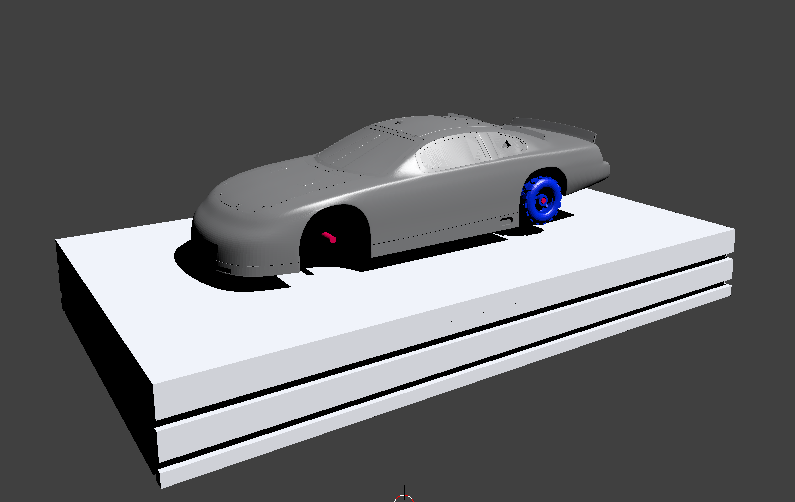
\includegraphics[width=0.8\textwidth ]{./images/BAT.png}
\caption{A example scene for the Basic Assembly Test. The actual car model may differ, but the wheels (\emph{blue}) need to be fitted onto the axes (\emph{red}).}
\label{fig:BAT_car}
\end{figure}


\subsection{Manipulation Objects}
The manipulation objects in this test may include the objects specified in Table \ref{tab:manipulation_objects}.
\todo{Why are the normal objects relevant for this task, if only wheels need to be fitted onto axes? (Fred)}
The set of objects is extended by:

\begin{table}[p]
\begin{tabular}{|c|c|c|p{5cm}|}
\hline 
 & Symbolic Description & Weight (in g) & Details \\ 
\hline 
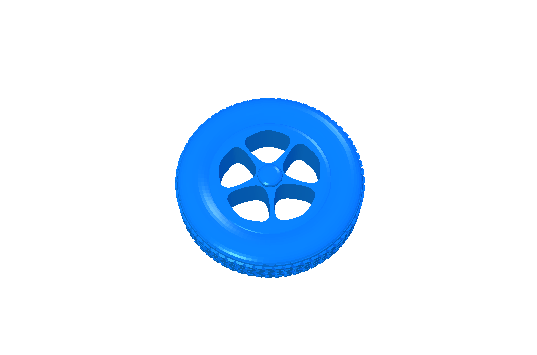
\includegraphics[width=3cm]{./images/BAT_Tire.png}  & T40 & approx. 50g & Height: 40mm \newline
 Width: 40mm \newline
 Length: approx. 10mm \\ 
\hline 
\end{tabular} 

\label{tab:bat_objects}
\caption{Examples of assembly objects}
\end{table}

All objects can be printed using a 3D-printer (e.g. axis and wheel), the car model is only for visualization purposes. All parts are available as STL files.

\subsection{Task}
A single robot is used. The task consists of a sequence of assembly operations, with a small base movement in between. The objective is to collect a set of objects and perform an assembly option. The robot will be given instruction where to pick up the wheels and where to assemble them. The task is to fit the wheels onto the axes. The wheels and the axes need to be detected by the robot. A few wheels may be already assembled. Therefore it is necessary to detect where a wheel is still missing.

\par
The task specification consists of: 
\begin{itemize}
	\item The specification of the initial place (e.g. D0, S5, U2) \todo{initial place of what? (Fred)}
	\item Location(s) of the wheels
	\item Location(s) where the assembly takes places
	\item The specification of a final place for the robot\todo{Do we really need this? I know this is also specified in the BMT, but ni the past we never used it. So, why to stick with it here? (Fred)}
\end{itemize}

\subsection{Rules}
The following rules have to be obeyed:

\begin{itemize}
\item The order in which the teams have to perform will be determined by a draw.
\item At the beginning of a team's period, the team will get the task specification. 
\item The team must set-up the robot in the designated start area.
\item A assembly object counts as successfully assembled when it is attached to the correct object or is in place for the external device to perform the assembly.
\item \todo{What about the maximum available time for the assembly? And how many assemblies need to be performed (Fred)}
\end{itemize}


\subsection{Scoring}
Points are awarded as follows:

\begin{itemize}
\item correct assembly:  \hfill 100 points
\item wrong assembly:  \hfill -100 points
\end{itemize}

\todo{Can you give an example for a wrong assembly. What's the objective of the penalty points, if you only get points for a correct assembly? (Fred)}

\todo{Why are we not using any of the objects from the RoboCup or RoCKIn set and introducing new objects instead. In my opinion increases the entry barrier for teams to participate in this challenge. (Fred)}
